\documentclass[letterpaper, titlepage, 10pt]{article}

\usepackage[margin=4cm]{geometry}
\usepackage[bookmarks]{hyperref} % wg. pdf indicies

\usepackage{listings} % wg. source listings

\usepackage{float} % wg. 'H' on figures (specify exact location)

\usepackage{tikz}
\usetikzlibrary{decorations.pathreplacing}
\usetikzlibrary{decorations.markings}
\usetikzlibrary{arrows}
\usetikzlibrary{positioning} % wg. 'of' relative positioning
\usetikzlibrary{shapes.misc} % wg. 'rounded rectangle'

% Styling to add arrows to paths
\tikzset{
  on each segment/.style={
    decorate,
    decoration={
      show path construction,
      moveto code={},
      lineto code={
        \path [#1]
        (\tikzinputsegmentfirst) -- (\tikzinputsegmentlast);
      },
      curveto code={
        \path [] (\tikzinputsegmentfirst)
        .. controls
        (\tikzinputsegmentsupporta) and (\tikzinputsegmentsupportb)
        ..
        (\tikzinputsegmentlast);
      },
      closepath code={
        \path [#1]
        (\tikzinputsegmentfirst) -- (\tikzinputsegmentlast);
      },
    },
  },
  % style to add an arrow in the middle of a path segment
  mid arrow/.style={
    postaction={
      decorate,
      decoration={
        markings,
        % Draw arrows manually to get them centered correctly, because this
        % isn't the default behavior for TIKZ
        mark=at position #1 with {
          \fill (2pt,0)--(-2pt,2.31pt)--(-2pt,-2.31pt)--cycle;
        }
      }
    }
  }
}

% path styling
\tikzset {
  syntax path/.style = {
    draw = black,
    rounded corners = 2mm
  },
  arrs/.style = {
    syntax path,
    postaction = {
      on each segment = {
        mid arrow = 0.5
      }
    }
  },
  % path style adds an arrow to each segment
  arr/.style = {
    syntax path,
    mid arrow = 0.5
  },
  % path style with no arrows
  narr/.style = {
    syntax path
  }
}

% node styling
\tikzset {
  syntax node/.style = {
    draw = black,
    inner sep = 0.2cm
  },
  % terminal symbol
  term/.style = {
    syntax node,
    rounded rectangle,
    font = \ttfamily
  },
  % non-terminal symbol
  nterm/.style = {
    syntax node,
    rectangle,
    font = \itshape
  },
  % support node
  entry/.style = {
    draw = black,
    circle,
    thick,
    minimum size = .2cm,
    inner sep = 0
  },
  exit/.style = {
    entry
  },
  node distance = 0.5cm
}

\title{Syntax Documentation}
\date{}

\begin{document}

\maketitle

\section{Primative Elements}

\subsection{Identifier}

\subsection{Right Identifier}

An identifier which may be used on the right side of a context.
This is the result of a normal identifier not including certain keywords, which may be valid in other contexts.

\begin{figure}[h]
  \centering
  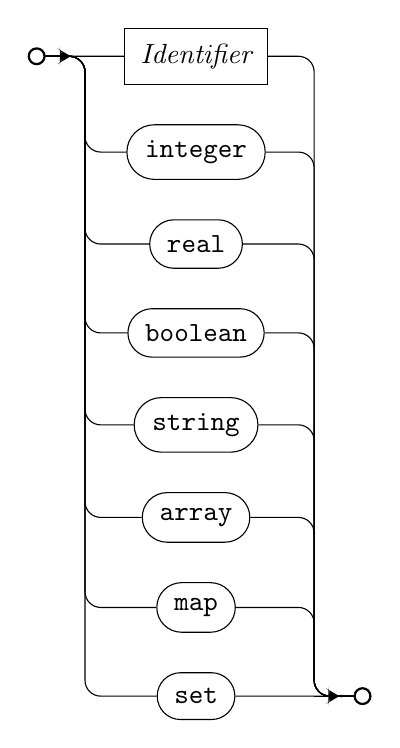
\begin{tikzpicture}
    \node[entry] (entry) {};
    \coordinate[right=of entry] (choice);
    \node[nterm] (id) [right=of choice] {Identifier};
    \node[term] (integer) [below=of id] {integer};
    \node[term] (real) [below=of integer] {real};
    \node[term] (boolean) [below=of real] {boolean};
    \node[term] (string) [below=of boolean] {string};
    \node[term] (array) [below=of string] {array};
    \node[term] (map) [below=of array] {map};
    \node[term] (set) [below=of map] {set};

    \coordinate[right=1cm of set] (aggr);
    \node[exit] (exit) [right=of aggr] {};

    \draw[narr] (entry) -- (id) -| (aggr) -- (exit);
    \draw[narr] (entry) -- (choice) |- (integer) -| (aggr) -- (exit);
    \draw[narr] (entry) -- (choice) |- (real) -| (aggr) -- (exit);
    \draw[narr] (entry) -- (choice) |- (boolean) -| (aggr) -- (exit);
    \draw[narr] (entry) -- (choice) |- (string) -| (aggr) -- (exit);
    \draw[narr] (entry) -- (choice) |- (array) -| (aggr) -- (exit);
    \draw[narr] (entry) -- (choice) |- (map) -| (aggr) -- (exit);
    \draw[narr] (entry) -- (choice) |- (set) -- (exit);

    \draw[arr] (entry) -- (choice);
    \draw[arr] (aggr) -- (exit);
  \end{tikzpicture}
\end{figure}

\subsection{String Literal}

A literal value representing a string. It should be noted that \textit{Character} is any UTF-8 character, as well as the standard escape characters. \textbf{WE NEED TO DEFINE STANDARD ESCAPE CHARACTERS AT SOME POINT}.

\begin{figure}[H]
  \centering

  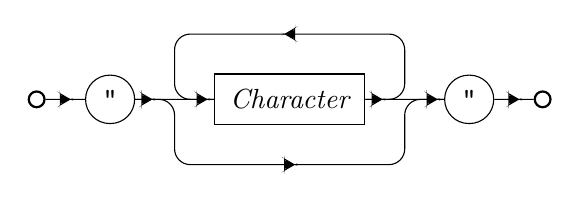
\begin{tikzpicture}
    \node[entry] (entry) {};
    \node[term] (quote) [right=of entry] {"};
    \coordinate [right=of quote] (quote-character);
    \node[nterm] (character) [right=of quote-character] {Character};
    \coordinate [right=of character] (character-endquote);
    \coordinate [above=of character] (character-above);
    \coordinate [below=of character] (character-below);
    \node[term] (endquote) [right=of character-endquote] {"};
    \node[exit] (exit) [right=of endquote] {};

    \draw[arrs] (entry)
    -- (quote)
    -- (quote-character)
    -- (character)
    -- (character-endquote)
    -- (endquote)
    -- (exit);

    \draw[arr] (character)
    -- (character-endquote)
    |- (character-above)
    -| (quote-character)
    -- (character);

    \draw[arr] (quote)
    -- (quote-character)
    |- (character-below)
    -| (character-endquote)
    -- (endquote);
  \end{tikzpicture}
\end{figure}


\subsection{Integer Literal}

A literal value representing an integer. \textit{Digit} is any single digit from the set \{0, 1, 2, 3, 4, 5, 6, 7, 8 , 9\}.

\begin{figure}[H]
  \centering
  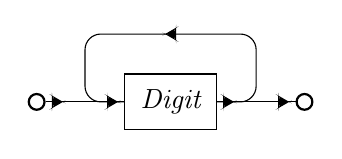
\begin{tikzpicture}
    \node[entry] (entry) {};
    \coordinate [right=of entry] (entry-digit);
    \node[nterm] (digit) [right=of entry-digit] {Digit};
    \coordinate [above=of digit] (digit-above);
    \coordinate [right=of digit] (digit-exit);
    \node[exit] (exit) [right=of digit-exit] {};

    \draw[arrs] (entry)
    -- (entry-digit)
    -- (digit)
    -- (digit-exit)
    -- (exit);
    \draw[arr] (digit)
    -- (digit-exit)
    |- (digit-above)
    -| (entry-digit)
    -- (digit);
  \end{tikzpicture}
\end{figure}

\subsection{Real Literal}

A literal value representing an real. \textit{Digit} is any single digit from the set \{0, 1, 2, 3, 4, 5, 6, 7, 8 , 9\}.

\begin{figure}[H]
  \centering
  \begin{tikzpicture}
    \node[entry] (entry) {};
    \coordinate [right=of entry] (entry-digit);
    \node[nterm] (digit) [right=of entry-digit] {Digit};
    \coordinate [above=of digit] (digit-above);
    \coordinate [below=of digit] (digit-below);
    \coordinate [right=of digit] (digit-decimal);
    \node[term] (decimal) [right=of digit-decimal] {.};
    \coordinate [right=of decimal] (decimal-digit);
    \node[nterm] (second-digit) [right=of decimal-digit] {Digit};
    \coordinate [above=of second-digit] (second-above);
    \coordinate [right=of second-digit] (second-exit);
    \node[exit] (exit) [right=of second-exit] {};

    \draw[arrs] (entry)
    -- (entry-digit)
    -- (digit)
    -- (digit-decimal)
    -- (decimal)
    -- (decimal-digit)
    -- (second-digit)
    -- (second-exit)
    -- (exit);

    \draw[arr] (digit)
    -- (digit-exit)
    |- (digit-above)
    -| (entry-digit)
    -- (digit);

    \draw[arr] (entry)
    -- (entry-digit)
    |- (digit-below)
    -| (digit-decimal)
    -- (decimal);

    \draw[arr] (second-digit)
    -- (second-exit)
    |- (second-above)
    -| (decimal-digit)
    -- (second-digit);
  \end{tikzpicture}
\end{figure}

\subsection{Boolean Literal}

A literal value representing a boolean.

\begin{figure}[H]
  \centering
  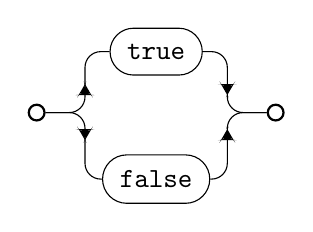
\begin{tikzpicture}
    \node[entry] (entry) {};
    \coordinate [right=of entry] (entry-list);
    \node[term] (false) [below right=.75cm of entry-list] {false};
    \node[term] (true) [above=1cm of false] {true};
    \coordinate [above right=.75cm of false] (list-exit);
    \node[exit] (exit) [right=of list-exit] {};

    \draw[arr] (entry) -- (entry-list) |- (true);
    \draw[arr] (entry) -- (entry-list) |- (false);
    \draw[arr] (true) -| (list-exit) -- (exit);
    \draw[arr] (false) -| (list-exit) -- (exit);
  \end{tikzpicture}
\end{figure}


\newpage
\section{Declaration Blocks}

\subsection{Program}

A full program; the entry point of a parse.

\begin{figure}[H]
  \centering

  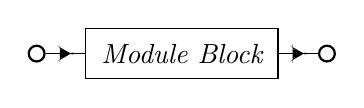
\begin{tikzpicture}
    \node[entry] (entry) {};
    \node[nterm] (mod) [right=of entry] {Module Block};
    \node[exit] (exit) [right=of mod] {};

    \draw[arr] (entry) -- (mod);
    \draw[arr] (mod) -- (exit);
  \end{tikzpicture}
\end{figure}

\subsection{Module Block}

One or more modules.

\begin{figure}[H]
  \centering
  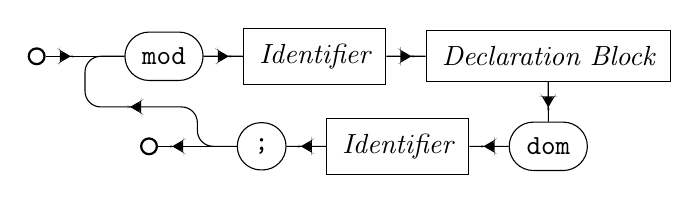
\begin{tikzpicture}
    \node[entry] (entry) {};
    \coordinate[right=of entry] (entry-mod);
    \node[term] (mod) [right=of entry-mod] {mod};
    \node[nterm] (name) [right=of mod] {Identifier};
    \node[nterm] (decl) [right=of name] {Declaration Block};
    \node[term] (dom) [below=of decl] {dom};
    \node[nterm] (exit name) [left=of dom] {Identifier};
    \node[term] (semi) [left=of exit name] {;};
    \coordinate[left=of semi] (semi-exit);
    \node[exit] (exit) [left=of semi-exit] {};

    \draw[arr] (entry) -- (entry-mod);
    \draw[narr] (entry-mod) -- (mod);

    \draw[arrs] (mod)
      -- (name)
      -- (decl)
      -- (dom)
      -- (exit name)
      -- (semi);

    \draw[narr] (semi) -- (semi-exit);
    \draw[arr] (semi-exit) -- (exit);

    \draw[arr] (semi)
      -- (semi-exit)
      -- ++(0, 0.5)
      -| (entry-mod)
      -- (mod);
  \end{tikzpicture}
\end{figure}

\subsection{Declaration Block}

A series of declarations

\begin{figure}[H]
  \centering
  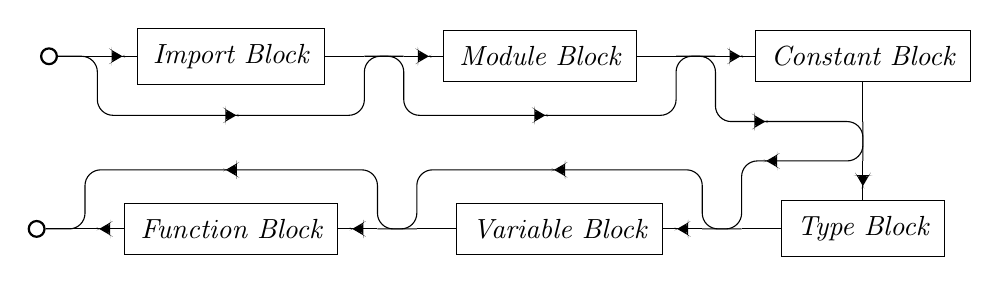
\begin{tikzpicture}
    \node[entry] (entry) {};
    \coordinate[right=of entry] (entry-imports);

    \node[nterm] (imports) [right=of entry-imports] {Import Block};
    \coordinate[right=of imports] (imports-mods 1);
    \coordinate[right=of imports-mods 1] (imports-mods 2);

    \node[nterm] (mods) [right=of imports-mods 2] {Module Block};
    \coordinate[right=of mods] (mods-consts 1);
    \coordinate[right=of mods-consts 1] (mods-consts 2);

    \node[nterm] (consts) [right=of mods-consts 2] {Constant Block};
    \coordinate[below=of consts] (consts-types 1);
    \coordinate[below=of consts-types 1] (consts-types 2);

    \node[nterm] (types) [below=of consts-types 2] {Type Block};
    \coordinate[left=of types] (types-vars 1);
    \coordinate[left=of types-vars 1] (types-vars 2);

    \node[nterm] (vars) [left=of types-vars 2] {Variable Block};
    \coordinate[left=of vars] (vars-funcs 1);
    \coordinate[left=of vars-funcs 1] (vars-funcs 2);

    \node[nterm] (funcs) [left=of vars-funcs 2] {Function Block};
    \coordinate[left=of funcs] (funcs-exit);

    \node[exit] (exit) [left=of funcs-exit] {};

    % main path
    \draw[narr] (entry) -- (entry-imports);
    \draw[arr] (entry-imports) -- (imports);
    
    \draw[narr] (imports) -- (imports-mods 1);
    \draw[arr] (imports-mods 2) -- (mods);

    \draw[narr] (mods) -- (mods-consts 1);
    \draw[arr] (mods-consts 2) -- (consts);

    \draw[narr] (consts) -- (consts-types 1);
    \draw[arr] (consts-types 2) -- (types);
      
    \draw[narr] (types) -- (types-vars 1);
    \draw[arr] (types-vars 2) -- (vars);

    \draw[narr] (vars) -- (vars-funcs 1);
    \draw[arr] (vars-funcs 2) -- (funcs);

    \draw[arr] (funcs) -- (funcs-exit);
    \draw[narr] (funcs-exit) -- (exit);
    
    % side path
    \draw[arr] (entry)
      -- (entry-imports)
      -- ++(0, -0.75)
      -| (imports-mods 1)
      -- (imports-mods 2);

    \draw[arr] (imports-mods 1)
      -- (imports-mods 2)
      -- ++(0, -0.75)
      -| (mods-consts 1)
      -- (mods-consts 2);

    \draw[arr] (mods-consts 1)
      -- (mods-consts 2)
      |- (consts-types 1)
      -- (consts-types 2);

    \draw[arr] (consts-types 1)
      -- (consts-types 2)
      -| (types-vars 1)
      -- (types-vars 2);

    \draw[arr] (types-vars 1)
      -- (types-vars 2)
      -- ++(0, 0.75)
      -| (vars-funcs 1)
      -- (vars-funcs 2);

    \draw[arr] (vars-funcs 1)
      -- (vars-funcs 2)
      -- ++(0, 0.75)
      -| (funcs-exit)
      -- (exit);
  \end{tikzpicture}
\end{figure}

\subsection{Import Block}

One or more import declarations.

\begin{figure}[H]
  \centering
  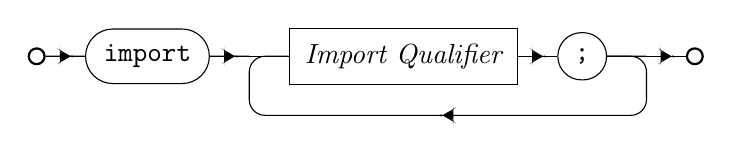
\begin{tikzpicture}
    \node[entry] (entry) {};
    \node[term] (import) [right=of entry] {import};
    \coordinate[right=of import] (import-qualifier);
    \node[nterm] (qualifier) [right=of import-qualifier] {Import Qualifier};
    \node[term] (semi) [right=of qualifier] {;};
    \coordinate[right=of semi] (semi-exit);
    \node[exit] (exit) [right=of semi-exit] {};

    \draw[arrs] (entry)
      -- (import)
      -- (import-qualifier);

    \draw[narr] (import-qualifier)
      -- (qualifier);

    \draw[arr] (qualifier) -- (semi);

    \draw[narr] (semi) -- (semi-exit);

    \draw[arr] (semi-exit) -- (exit);

    \draw[arr] (semi)
      -- (semi-exit)
      -- ++(0, -0.75)
      -| (import-qualifier)
      -- (qualifier);
  \end{tikzpicture}
\end{figure}

\subsubsection{Import Qualifier}

A qualifying series of identifiers for a module.

\begin{figure}[H]
  \centering
  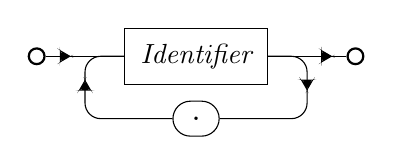
\begin{tikzpicture}
    \node[entry] (entry) {};
    \coordinate[right=of entry] (entry-name);
    \node[nterm] (name) [right=of entry-name] {Identifier};
    \coordinate[right=of name] (name-exit);
    \node[exit] (exit) [right=of name-exit] {};

    \node[term, node distance = 0.2cm] (dot) [below=of name] {.};

    \draw[arr] (entry) -- (entry-name);
    
    \draw[narr] (entry-name)
      -- (name)
      -- (name-exit);

    \draw[arr] (name-exit) -- (exit);

    \draw[narr, mid arrow = 0.35] (name)
      -- (name-exit)
      |- (dot);

    \draw[narr, mid arrow = 0.65] (dot)
      -| (entry-name)
      -- (name);
  \end{tikzpicture}
\end{figure}

\subsection{Constant Block}

One or more constant declarations.

\begin{figure}[H]
  \centering
  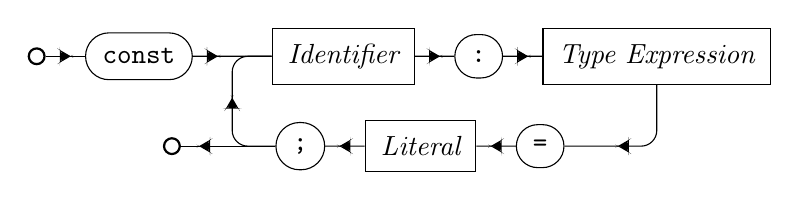
\begin{tikzpicture}
    \node[entry] (entry) {};
    \node[term] (const) [right=of entry] {const};
    \coordinate[right=of const] (const-name);
    \node[nterm] (name) [right=of const-name] {Identifier};
    \node[term] (colon) [right=of name] {:};
    \node[nterm] (type) [right=of colon] {Type Expression};
    \node[term] (eq) [below left=0.5cm and 0cm of type] {=};
    \node[nterm] (literal) [left=of eq] {Literal};
    \node[term] (semi) [left=of literal] {;};
    \node[exit] (exit) [left=1.2cm of semi] {};

    \draw[arrs] (entry) -- (const);
    \draw[narr, mid arrow = 0.25] (const) -- (name);
    \draw[arrs] (name)
      -- (colon)
      -- (type);

    \draw[narr, mid arrow = 0.6] (type) |- (eq);

    \draw[arrs] (eq)
      -- (literal)
      -- (semi);

    \draw[narr, mid arrow = 0.75] (semi) -- (exit);
    
    \draw[arr] (semi) -| (const-name) -- (name);

  \end{tikzpicture}
\end{figure}

\subsection{Variable Block}

One or more variable declarations.

\begin{figure}[H]
  \centering
  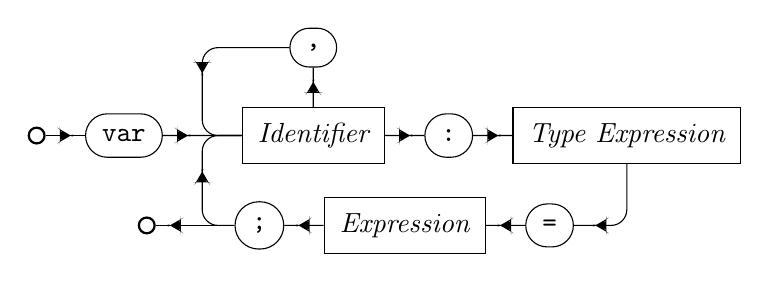
\begin{tikzpicture}
    \node[entry] (entry) {};
    \node[term] (var) [right=of entry] {var};
    \coordinate[right=of var] (var-name);
    \node[nterm] (name) [right=of var-name] {Identifier};
    \node[term] (comma) [above=of name] {,};
    \node[term] (colon) [right=of name] {:};
    \node[nterm] (type) [right=of colon] {Type Expression};
    \node[term] (eq) [below left=0.5cm and -0.5cm of type] {=};
    \node[nterm] (expr) [left=of eq] {Expression};
    \node[term] (semi) [left=of expr] {;};
    \node[exit] (exit) [left=1cm of semi] {};
    
    \draw[arrs] (entry) -- (var);
    \draw[narr, mid arrow = 0.25] (var) -- (name);
    \draw[arrs] (name)
      -- (colon)
      -- (type);

    \draw[arr] (name) -- (comma) ;
    \draw[arr] (comma) -| (var-name) -- (name);

    \draw[narr, mid arrow = 0.75] (type) |- (eq);

    \draw[arrs] (eq)
      -- (expr)
      -- (semi);

    \draw[narr, mid arrow = 0.75] (semi) -- (exit);
    
    \draw[arr] (semi) -| (var-name) -- (name);

  \end{tikzpicture}
\end{figure}

\subsection{Type Block}

One or more type declarations

\begin{figure}[H]
  \centering
  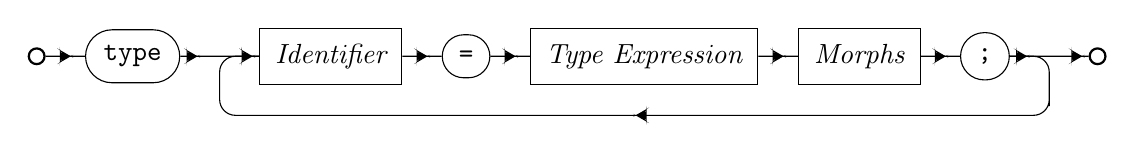
\begin{tikzpicture}
    \node[entry] (entry) {};
    \node[term] (type) [right=of entry] {type};
    \coordinate [right=of type] (type-name);
    \node[nterm] (name) [right=of type-name] {Identifier};
    \node[term] (equals) [right=of name] {=};
    \node[nterm] (typexp) [right=of equals] {Type Expression};
    \node[nterm] (morphs) [right=of typexp] {Morphs};
    \node[term] (semi) [right=of morphs] {;};
    \coordinate[right=of semi] (semi-exit);
    \node[exit] (exit) [right=of semi-exit] {};

    \draw[arrs] (entry)
    -- (type)
    -- (type-name)
    -- (name)
    -- (equals)
    -- (typexp)
    -- (morphs)
    -- (semi)
    -- (semi-exit)
    -- (exit);

    \draw[arr] (semi)
    -- (semi-exit)
    |- ++(0, -.75)
    -| (type-name)
    -- (name);
  \end{tikzpicture}
\end{figure}

\newpage
\section{Types}

\subsection{Type Expression}

Specifying a type.

\begin{figure}[H]
  \centering
  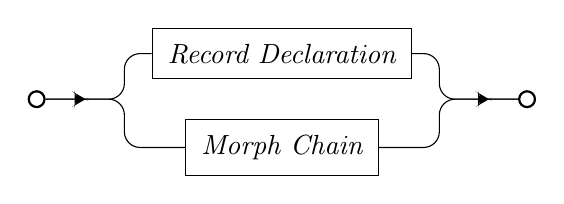
\begin{tikzpicture}
    \coordinate (mid);
    \coordinate[left=2cm of mid] (left);
    \coordinate[right=2cm of mid] (right);

    \node[entry] (entry) [left=1cm of left] {};
    \node[exit] (exit) [right=1cm of right] {};

    \node[nterm] (rec) [above=0.25cm of mid] {Record Declaration};
    \node[nterm] (morph) [below=0.25cm of mid] {Morph Chain};

    \draw[narr, mid arrow = 0.25] (entry) -- (left) |- (rec);
    \draw[narr] (entry) -- (left) |- (morph);

    \draw[narr, mid arrow = 0.75] (rec) -| (right) -- (exit);
    \draw[narr] (morph) -| (right) -- (exit);
  \end{tikzpicture}
\end{figure}

\subsection{Record Declaration}

The specification of a record's layout.

\begin{figure}[H]
  \centering
  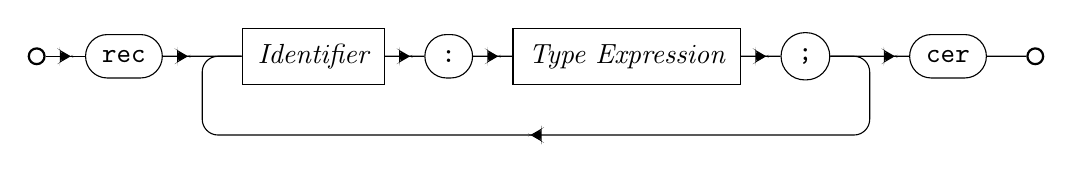
\begin{tikzpicture}
    \node[entry] (entry) {};
    \node[term] (rec) [right=of entry] {rec};
    \coordinate[right=of rec] (rec-id);
    \node[nterm] (id) [right=of rec-id] {Identifier};
    \node[term] (colon) [right=of id] {:};
    \node[nterm] (type) [right=of colon] {Type Expression};
    \node[term] (semi) [right=of type] {;};
    \coordinate[right=of semi] (semi-cer);
    \node[term] (cer) [right=of semi-cer] {cer};
    \node[exit] (exit) [right=of cer] {};

    \draw[arr] (entry) -- (rec);
    \draw[narr, mid arrow = 0.25] (rec) -- (id);
    \draw[arrs] (id) -- (colon) -- (type) -- (semi);
    \draw[narr, mid arrow = 0.75] (semi) -- (cer);
    \draw[narr] (cer) -- (exit);
    \draw[arr] (semi) -- (semi-cer) -- ++(0, -1) -| (rec-id) -- (id);
  \end{tikzpicture}
\end{figure}

\subsection{Morph Chain}

A specification of a morph path. May be used for explicit morphs or as a type.

\begin{figure}[H]
  \centering
  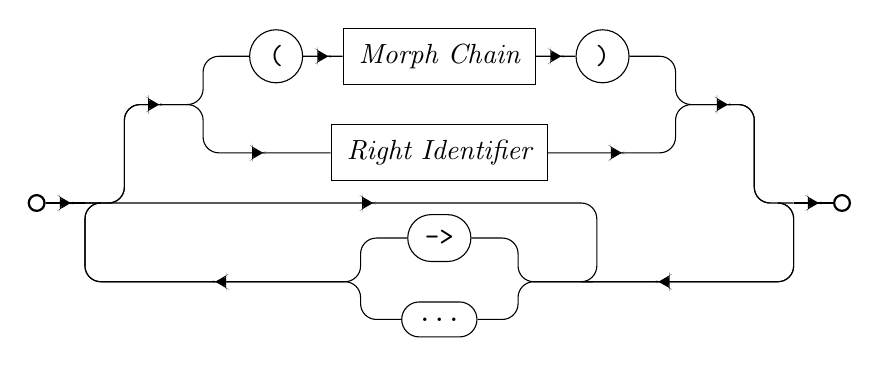
\begin{tikzpicture}
    \coordinate (mid);
    \coordinate[above=1.25cm of mid] (top);
    \coordinate[below=1cm of mid] (bot);

    \coordinate[left=3cm of top] (top-left);
    \coordinate[right=3cm of top] (top-right);

    \coordinate[left=1cm of bot] (bot-left);
    \coordinate[right=1cm of bot] (bot-right);
    \coordinate[right=2cm of bot] (bot-right-right);

    \coordinate[left=4cm of mid] (entry-choices);
    \coordinate[left=of entry-choices] (entry-loop);
    \node[entry] (entry) [left=of entry-loop] {};

    \coordinate[right=4cm of mid] (exit-choices);
    \coordinate[right=of exit-choices] (exit-loop);
    \node[exit] (exit) [right=of exit-loop] {};

    \node[nterm] (id) [below=0.25cm of top] {Right Identifier};

    \node[nterm] (inner) [above=0.25cm of top] {Morph Chain};
    \node[term] (lparen) [left=of inner] {(};
    \node[term] (rparen) [right=of inner] {)};

    \node[term] (dotdot) [above=0.25cm of bot] {->};
    \node[term] (dotdotdot) [below=0.25cm of bot] {...};

    \draw [arr] (entry) -| (bot-right-right) -- +(-0.05, 0);

    \draw [arr] (entry) -- (entry-loop);

    \draw [arr]
      (entry-choices) + (-0.2, 0)
      -- (entry-choices)
      |- (top-left)
      |- (lparen);

    \draw [narr, mid arrow = 0.8]
      (entry-loop)
      -- (entry-choices)
      |- (top-left)
      |- (id);

    \draw [narr, mid arrow = 0.45]
      (rparen)
      -| (top-right)
      -| (exit-choices)
      -- (exit-loop);

    \draw [narr, mid arrow = 0.2]
      (id)
      -| (top-right)
      -| (exit-choices)
      -- ++(0.2, 0);

    \draw [arr]
      (dotdot)
      -| (bot-left)
      -| (entry-loop)
      -- ++(0.2, 0);

    \draw [narr]
      (dotdotdot)
      -| (bot-left)
      -| (entry-loop)
      -- ++(0.2, 0);

    \draw [narr]
      (exit-loop) + (-0.2, 0)
      -- (exit-loop)
      |- (bot-right)
      |- (dotdot);

    \draw [arr]
      (exit-loop) + (-0.2, 0)
      -- (exit-loop)
      |- (bot-right)
      |- (dotdotdot);

    \draw [arr] (exit-loop) -- (exit);

    \draw [arrs] (lparen) -- (inner) -- (rparen);
  \end{tikzpicture}
\end{figure}

\newpage
\section{Functions}

\subsection{Function Block}

A declaration of a function.

\begin{figure}[H]
  \centering
  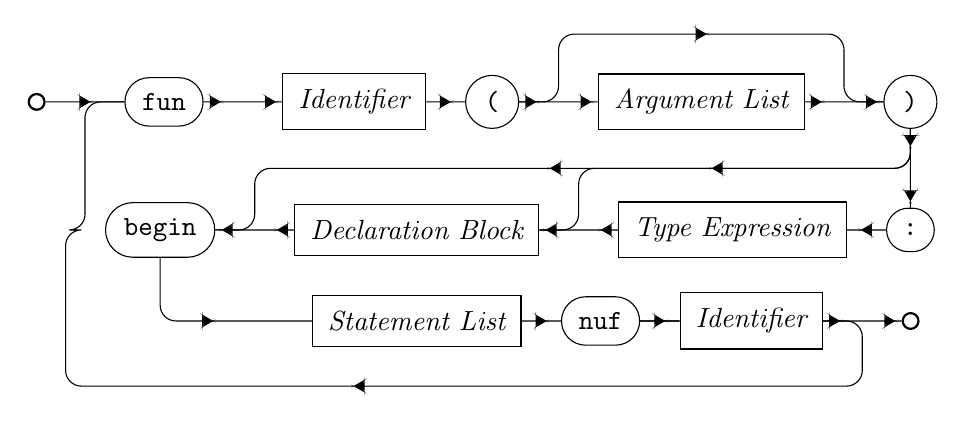
\begin{tikzpicture}
    \node[entry] (entry) {};
    \coordinate [right=of entry] (entry-fun);
    \node[term] (fun) [right=of entry-fun] {fun};
    \coordinate [right=of fun] (fun-name);
    \node[nterm] (name) [right=of fun-name] {Identifier};
    \node[term] (open-paren) [right=of name] {(};
    \coordinate [right=of open-paren] (paren-args);
    \node[nterm] (args) [right=of paren-args] {Argument List};
    \coordinate [above=of args] (args-above);
    \coordinate [right=of args] (args-paren);
    \node[term] (close-paren) [right=of args-paren] {)};
    \coordinate [below=of close-paren] (paren-below);
    \node[term] (colon) [below=of paren-below] {:};
    \node[nterm] (return-type) [left=of colon] {Type Expression};
    \coordinate [left=of return-type] (type-decl);
    \node[nterm] (declarations) [left=of type-decl] {Declaration Block};
    \coordinate [left=of declarations] (decl-begin);
    \node[term] (begin) [left=of decl-begin] {begin};
    \coordinate [left=of begin] (begin-left);
    \coordinate [above=of begin] (begin-above);
    \node[nterm] (statements) [below=of declarations] {Statement List};
    \coordinate [below=of statements] (statements-below);
    \node[term] (end) [right=of statements] {nuf};
    \node[nterm] (name-close) [right=of end] {Identifier};
    \coordinate [right=of name-close] (name-exit);
    \node[exit] (exit) [right=of name-exit] {};

    \draw[arrs] (entry)
    -- (fun)
    -- (fun-name)
    -- (name)
    -- (open-paren)
    -- (paren-args)
    -- (args)
    -- (args-paren)
    -- (close-paren);

    \draw[arr] (open-paren)
    -- (paren-args)
    |- (args-above)
    -| (args-paren)
    -- (close-paren);

    \draw[arrs] (close-paren)
    -- (paren-below)
    -- (colon)
    -- (return-type)
    -- (type-decl)
    -- (declarations)
    -- (decl-begin)
    -- (begin);

    \draw[arr] (close-paren)
    -- (paren-below)
    -| (type-decl)
    -- (declarations);

    \draw[arr] (close-paren)
    -- (paren-below)
    -| (decl-begin)
    -- (begin);

    \draw[arr] (begin)
    |- (statements);

    \draw[arrs] (statements)
    -- (end)
    -- (name-close)
    -- (name-exit)
    -- (exit);

    \draw[arr] (end)
    -- (name-close)
    -- (name-exit)
    |- (statements-below)
    -| (begin-left)
    -| (entry-fun)
    -- (fun);
  \end{tikzpicture}
\end{figure}

\subsection{Argument List}

A list of arguments to a function.

\begin{figure}[H]
  \centering
  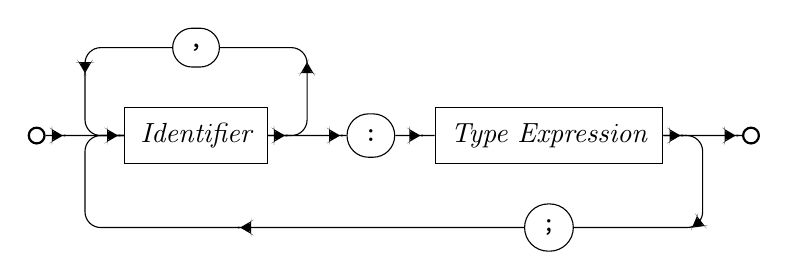
\begin{tikzpicture}
    \node[entry] (entry) {};
    \coordinate [right=of entry] (entry-name);
    \node[nterm] (name) [right=of entry-name] {Identifier};
    \node[term] (comma) [above=of name] {,};
    \coordinate [right=of name] (name-colon);
    \node[term] (colon) [right=of name-colon] {:};
    \node[nterm] (type) [right=of colon] {Type Expression};
    \coordinate [right=of type] (type-exit);
    \node[exit] (exit) [right=of type-exit] {};
    \node[term] (semicolon) [below=of type] {;};

    \draw[arrs] (entry)
    -- (entry-name)
    -- (name)
    -- (name-colon)
    -- (colon)
    -- (type)
    -- (type-exit)
    -- (exit);

    \draw[arr] (name)
    -- (name-colon)
    |- (comma);

    \draw[arr] (comma)
    -| (entry-name)
    -- (name);

    \draw[arr] (type)
    -- (type-exit)
    |- (semicolon);

    \draw[arr] (semicolon)
    -| (entry-name)
    -- (name);
  \end{tikzpicture}
\end{figure}

\newpage
\section{Statements}

\subsection{Statement List}

Sequential statements.

\begin{figure}[H]
  \centering
  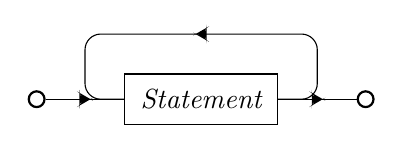
\begin{tikzpicture}
    \node[entry] (entry) {};
    \coordinate [right=of entry] (entry-statements);
    \node[nterm] (statement) [right=of entry-statements] {Statement};
    \coordinate [right=of statement] (statements-exit);
    \coordinate [above=of statement] (statement-above);
    \node[exit] (exit) [right=of statements-exit] {};

    \draw[arr] (entry)
    -- (entry-statements)
    -- (statement);

    \draw[arr] (statement)
    -- (statements-exit)
    -- (exit);

    \draw[arr] (statement)
    -- (statements-exit)
    |- (statement-above)
    -| (entry-statements)
    -- (statement);
  \end{tikzpicture}
\end{figure}

\subsection{Statement}

A singular statement.

\begin{figure}[H]
  \centering
  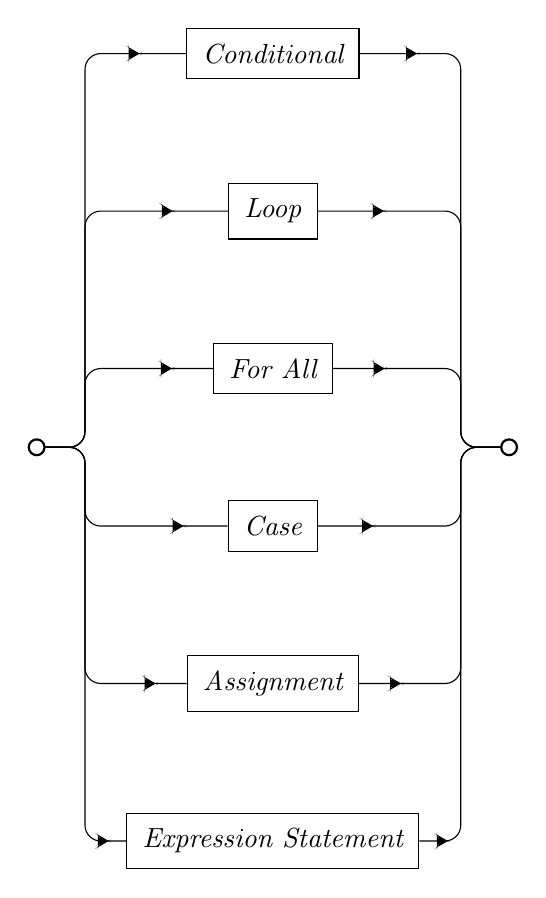
\begin{tikzpicture}
    \node[entry] at (-3, 0) (entry) {};
    \coordinate [right=of entry] (entry-list);
    \node[exit] at (3, 0) (exit)  {};
    \coordinate [left=of exit] (list-exit);
    \node[nterm] at (0, 1) (fa)  {For All};
    \node[nterm] at (0, 3) (loop)  {Loop};
    \node[nterm] at (0, 5) (if)  {Conditional};
    \node[nterm] at (0, -1) (case)  {Case};
    \node[nterm] at (0, -3) (assign)  {Assignment};
    \node[nterm] at (0, -5) (expr)  {Expression Statement};

    \draw[narr, mid arrow = 0.9] (entry)
    -- (entry-list)
    |- (if);
    \draw[narr, mid arrow = 0.85] (entry)
    -- (entry-list)
    |- (loop);
    \draw[narr, mid arrow = 0.8] (entry)
    -- (entry-list)
    |- (fa);
    \draw[narr, mid arrow = 0.8] (entry)
    -- (entry-list)
    |- (case);
    \draw[narr, mid arrow = 0.9] (entry)
    -- (entry-list)
    |- (assign);
    \draw[narr, mid arrow = 0.95] (entry)
    -- (entry-list)
    |- (expr);

    \draw[narr, mid arrow = 0.1] (if)
    -| (list-exit)
    -- (exit);
    \draw[narr, mid arrow = 0.15] (loop)
    -| (list-exit)
    -- (exit);
    \draw[narr, mid arrow = 0.2] (fa)
    -| (list-exit)
    -- (exit);
    \draw[narr, mid arrow = 0.2] (case)
    -| (list-exit)
    -- (exit);
    \draw[narr, mid arrow = 0.1] (assign)
    -| (list-exit)
    -- (exit);
    \draw[narr, mid arrow = 0.05] (expr)
    -| (list-exit)
    -- (exit);
  \end{tikzpicture}
\end{figure}

\subsection{Conditional}

Conditional statement.

\begin{figure}[H]
  \centering
  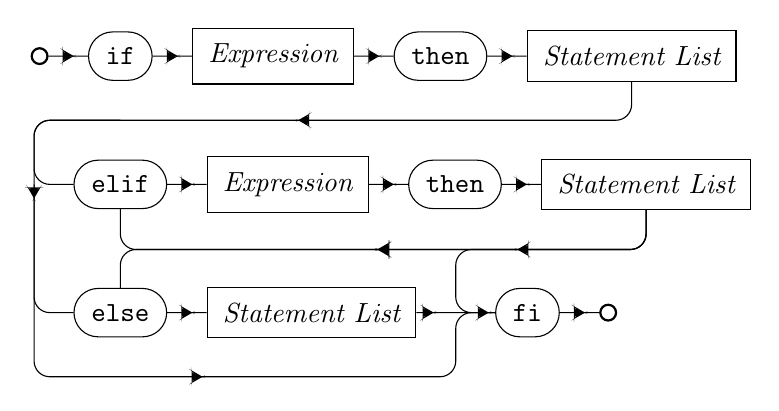
\begin{tikzpicture}
    \node[entry] (entry) {};
    \node[term] (if) [right=of entry] {if};
    \node[nterm] (if-expr) [right=of if] {Expression};
    \node[term] (if-then) [right=of if-expr] {then};
    \node[nterm] (if-statements) [right=of if-then] {Statement List};
    \coordinate [below=of if] (if-below);
    \node[term] (elif) [below=of if-below] {elif};
    \coordinate [left=of elif] (elif-left);
    \node[nterm] (elif-expr) [right=of elif] {Expression};
    \node[term] (elif-then) [right=of elif-expr] {then};
    \node[nterm] (elif-statements) [right=of elif-then] {Statement List};
    \coordinate [below=of elif-statements] (elif-statements-below);
    \coordinate [below=of elif] (elif-below);
    \node[term] (else) [below=of elif-below] {else};
    \coordinate [below=of else] (else-below);
    \coordinate [left=of else] (else-left);
    \node[nterm] (else-statements) [right=of else] {Statement List};
    \coordinate [right=of else-statements] (statements-fi);
    \node[term] (fi) [right=of statements-fi] {fi};
    \node[exit] (exit) [right=of fi] {};

    \draw[arrs] (entry)
    -- (if)
    -- (if-expr)
    -- (if-then)
    -- (if-statements);

    \draw[arrs] (elif)
    -- (elif-expr)
    -- (elif-then)
    -- (elif-statements);

    \draw[arrs] (else)
    -- (else-statements)
    -- (statements-fi)
    -- (fi)
    -- (exit);

    \draw[arr] (if-statements)
    |- (if-below)
    -| (elif-left)
    -- (elif);

    \draw[arr] (if-below)
    -| (elif-left)
    |- (else);

    \draw[arr] (elif-left)
    |- (else-below)
    -| (statements-fi)
    -- (fi);

    \draw[arr] (elif-statements)
    -- (elif-statements-below)
    -| (statements-fi)
    -- (fi);

    \draw[arr] (elif-statements)
    -- (elif-statements-below)
    -| (elif);

    \draw[arr] (elif-statements)
    -- (elif-statements-below)
    -| (else);
  \end{tikzpicture}
\end{figure}

\subsection{Loop Statement}

Basic loop. The only way to exit is to use a \textit{Break} statement.

\begin{figure}[H]
  \centering
  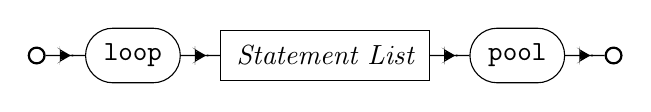
\begin{tikzpicture}
    \node[entry] (entry) {};
    \node[term] (loop) [right=of entry] {loop};
    \node[nterm] (statements) [right=of loop] {Statement List};
    \node[term] (pool) [right=of statements] {pool};
    \node[exit] (exit) [right=of pool] {};

    \draw[arrs] (entry)
    -- (loop)
    -- (statements)
    -- (pool)
    -- (exit);
  \end{tikzpicture}
\end{figure}

\subsection{Case Statement}

Case statement.

\begin{figure}[H]
  \centering
  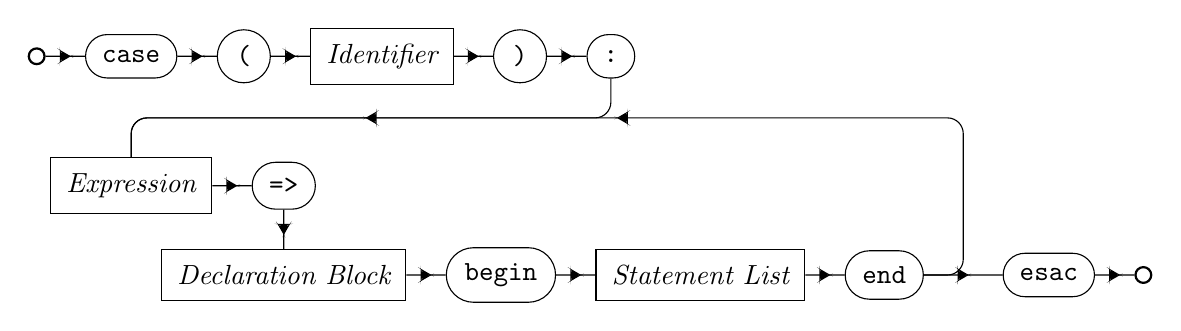
\begin{tikzpicture}
    \node[entry] (entry) {};
    \node[term] (case) [right=of entry] {case};
    \node[term] (open) [right=of case] {(};
    \node[nterm] (case-var) [right=of open] {Identifier};
    \node[term] (close) [right=of case-var] {)};
    \node[term] (colon) [right=of close] {:};
    \coordinate [below=of case] (case-below);
    \node[nterm] (expr) [below=of case-below] {Expression};
    \node[term] (arrow) [right=of expr] {=>};
    \node[nterm] (decl) [below=of arrow] {Declaration Block};
    \node[term] (begin) [right=of decl] {begin};
    \node[nterm] (statements) [right=of begin] {Statement List};
    \node[term] (end) [right=of statements] {end};
    \coordinate [right=of end] (end-esac);
    \node[term] (esac) [right=of end-esac] {esac};
    \node[exit] (exit) [right=of esac] {};

    \draw[arrs] (entry) -- (case) -- (open) -- (case-var) -- (close) -- (colon);
    \draw[arr] (colon) |- (case-below) -- (expr);
    \draw[arrs] (expr) -- (arrow) -- (decl) -- (begin) -- (statements) -- (end);
    \draw[arrs] (end) -- (esac) -- (exit);
    \draw[arr] (end) -- (end-esac) |- (case-below) -- (expr);
  \end{tikzpicture}
\end{figure}

\subsection{Assignment}

Assign a value to a variable or field of a record.

\begin{figure}[H]
  \centering
  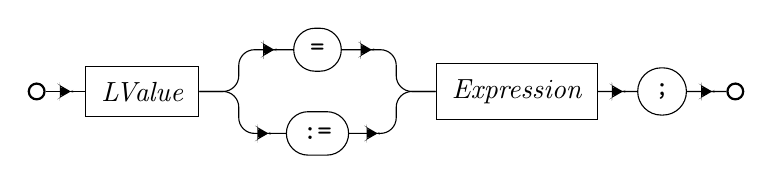
\begin{tikzpicture}
    \node[entry] (entry) {};
    \node[nterm] (left-side) [right=of entry] {LValue};
    \coordinate [right=of left-side] (left-assign);
    \coordinate [right=1cm of left-assign] (assign);
    \node[term] (shallow) [above=0.25cm of assign] {=};
    \node[term] (deep) [below=0.25cm of assign] {:=};
    \coordinate [right=1cm of assign] (assign-expr);
    \node[nterm] (expr) [right=of assign-expr] {Expression};
    \node[term] (semicolon) [right=of expr] {;};
    \node[exit] (exit) [right=of semicolon] {};

    \draw[arr] (entry) -- (left-side);
    \draw[narr, mid arrow = 0.8] (left-side) -- (left-assign) |- (shallow);
    \draw[narr, mid arrow = 0.8] (left-side) -- (left-assign) |- (deep);
    \draw[narr, mid arrow = 0.2] (shallow) -| (assign-expr) -- (expr);
    \draw[narr, mid arrow = 0.2] (deep) -| (assign-expr) -- (expr);
    \draw[arrs] (expr) -- (semicolon) -- (exit);
  \end{tikzpicture}
\end{figure}

\subsection{LValue}

Possible value on the left side of an assignment.

TODO: We need to talk about this in further detail.

\begin{figure}[H]
  \centering
  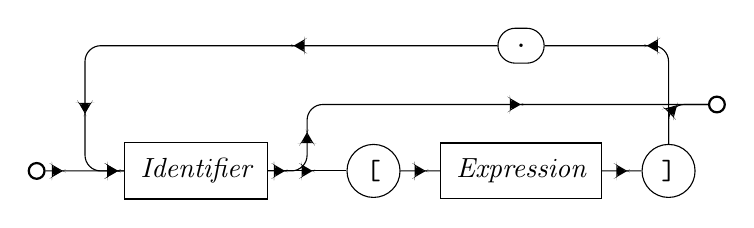
\begin{tikzpicture}
    \node[entry] (entry) {};
    \coordinate [right=of entry] (entry-id);
    \node[nterm] (id) [right=of entry-id] {Identifier};
    \coordinate [right=of id] (id-bracket);
    \coordinate [above=of id-bracket] (id-bracket-above);
    \node[term] (left) [right=of id-bracket] {[};
    \node[nterm] (expr) [right=of left] {Expression};
    \node[term] (right) [right=of expr] {]};
    \coordinate [above=of expr] (expr-dot);
    \node[term] (dot) [above=of expr-dot] {.};
    \coordinate [above=of right] (right-above);
    \node[exit] (exit) [right=of right-above] {};
    \coordinate [right=of exit] (exit-right);

    \draw[arrs] (entry) -- (entry-id) -- (id) -- (id-bracket) |- (exit);
    \draw[arrs] (dot) -| (entry-id) -- (id);
    \draw[arrs] (left) -- (expr) -- (right);
    \draw[arr] (right) |- (exit);
    \draw[arr] (right) |- (dot);
    \draw[arr] (id) -- (left);
  \end{tikzpicture}
\end{figure}

\subsection{Expression Statement}

A statement that evaluates an expression.

\begin{figure}[H]
  \centering
  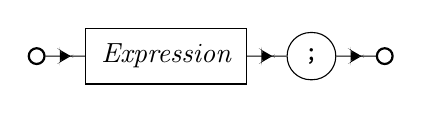
\begin{tikzpicture}
    \node[entry] (entry) {};
    \node[nterm] (expr) [right=of entry] {Expression};
    \node[term] (semicolon) [right=of expr] {;};
    \node[exit] (exit) [right=of semicolon] {};

    \draw[arrs] (entry) -- (expr) -- (semicolon) -- (exit);
  \end{tikzpicture}
\end{figure}

\newpage
\section{Expressions}

\subsection{Expression}

There are various types of expressions that can be evaluated.

\begin{figure}[H]
  \centering
  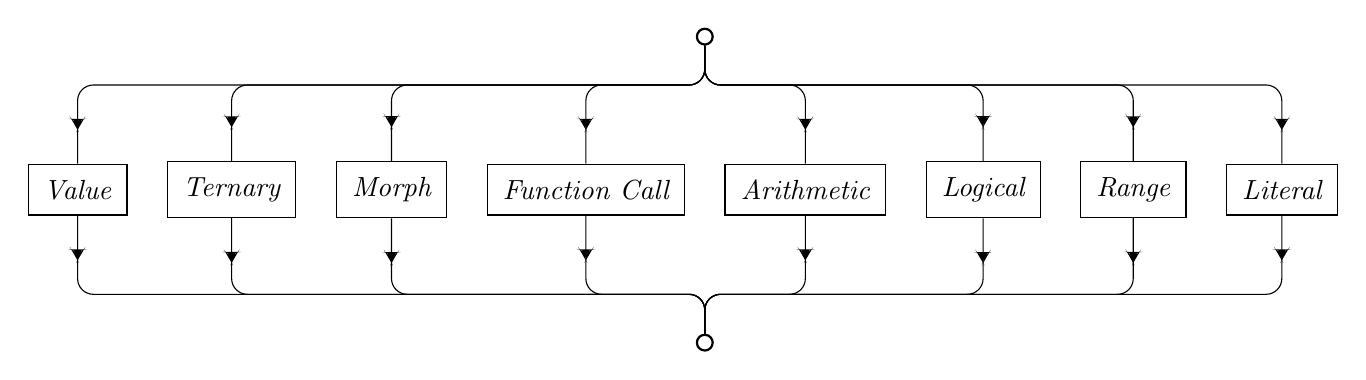
\begin{tikzpicture}
    \node[entry] (entry) {};
    \coordinate [below=of entry] (entry-list);
    \node[nterm] (arithmetic) [below right=1cm and .25cm of entry-list] {Arithmetic};
    \node[nterm] (func-call) [below left=1cm and .25cm of entry-list] {Function Call};
    \node[nterm] (logical) [right=of arithmetic] {Logical};
    \node[nterm] (range) [right=of logical] {Range};
    \node[nterm] (morph) [left=of func-call] {Morph};
    \node[nterm] (ternary) [left=of morph] {Ternary};
    \node[nterm] (value) [left=of ternary] {Value};
    \node[nterm] (literal) [right=of range] {Literal};
    \coordinate [below right=1cm and .25cm of func-call] (list-exit);
    \node[exit] (exit) [below=of list-exit] {};

    \draw[narr, mid arrow = -0.5cm] (entry) -- (entry-list) -| (func-call);
    \draw[narr, mid arrow = -0.5cm] (entry) -- (entry-list) -| (morph);
    \draw[narr, mid arrow = -0.5cm] (entry) -- (entry-list) -| (ternary);
    \draw[narr, mid arrow = -0.5cm] (entry) -- (entry-list) -| (value);
    \draw[narr, mid arrow = -0.5cm] (entry) -- (entry-list) -| (arithmetic);
    \draw[narr, mid arrow = -0.5cm] (entry) -- (entry-list) -| (logical);
    \draw[narr, mid arrow = -0.5cm] (entry) -- (entry-list) -| (range);
    \draw[narr, mid arrow = -0.5cm] (entry) -- (entry-list) -| (literal);

    \draw[narr, mid arrow = 0.5cm] (func-call)  |- (list-exit) -- (exit);
    \draw[narr, mid arrow = 0.5cm] (morph)      |- (list-exit) -- (exit);
    \draw[narr, mid arrow = 0.5cm] (ternary)    |- (list-exit) -- (exit);
    \draw[narr, mid arrow = 0.5cm] (value)      |- (list-exit) -- (exit);
    \draw[narr, mid arrow = 0.5cm] (arithmetic) |- (list-exit) -- (exit);
    \draw[narr, mid arrow = 0.5cm] (logical)    |- (list-exit) -- (exit);
    \draw[narr, mid arrow = 0.5cm] (range)      |- (list-exit) -- (exit);
    \draw[narr, mid arrow = 0.5cm] (literal)    |- (list-exit) -- (exit);

  \end{tikzpicture}
\end{figure}

\subsection{Literal Expression}

An expression that immediately evaluates to a literal value.

\begin{figure}[H]
  \centering
  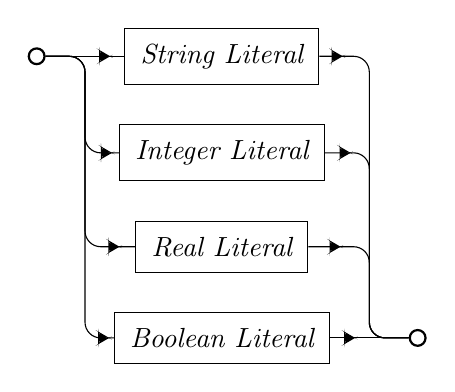
\begin{tikzpicture}
    \node[entry] (entry) {};
    \coordinate [right=of entry] (entry-list);
    \node[nterm] (string) [right=of entry-list] {String Literal};
    \node[nterm] (integer) [below=of string] {Integer Literal};
    \node[nterm] (real) [below=of integer] {Real Literal};
    \node[nterm] (boolean) [below=of real] {Boolean Literal};
    \coordinate [right=of boolean] (list-exit);
    \node[exit] (exit) [right=of list-exit] {};

    \draw[narr, mid arrow = 0.75] (entry) -- (string);
    \draw[narr, mid arrow = 0.25] (boolean) -- (exit);
    \draw[narr, mid arrow = 0.92] (entry) -- (entry-list) |- (integer);
    \draw[narr, mid arrow = 0.92] (entry) -- (entry-list) |- (real);
    \draw[narr, mid arrow = 0.97] (entry) -- (entry-list) |- (boolean);

    \draw[narr, mid arrow = 0.05] (string) -| (list-exit) -- (exit);
    \draw[narr, mid arrow = 0.08] (integer) -| (list-exit) -- (exit);
    \draw[narr, mid arrow = 0.15] (real) -| (list-exit) -- (exit);
  \end{tikzpicture}
\end{figure}

\subsection{Function Call}

Call a function with or without arguments.

\begin{figure}[H]
  \centering
  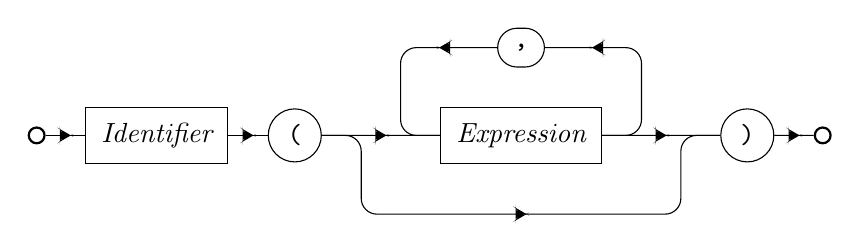
\begin{tikzpicture}
    \node[entry] (entry) {};
    \node[nterm] (name) [right=of entry] {Identifier};
    \node[term] (open) [right=of name] {(};
    \coordinate [right=of open] (open-loop);
    \coordinate [right=of open-loop] (loop-expr);
    \node[nterm] (expr) [right=of loop-expr] {Expression};
    \node[term] (comma) [above=of expr] {,};
    \coordinate [right=of expr] (expr-loop); 
    \coordinate [right=of expr-loop] (loop-close); 
    \node[term] (close) [right=of loop-close] {)};
    \node[exit] (exit) [right=of close] {};

    \draw[arrs] (entry) -- (name) -- (open);
    \draw[arrs] (open) -- (expr) -- (close);
    \draw[arr] (close) -- (exit);
    \draw[arr] (open) -- (open-loop) -- ++(0, -1) -| (loop-close) -- (close);
    \draw[narr, mid arrow = 0.75] (expr) -- (expr-loop) |- (comma);
    \draw[narr, mid arrow = 0.25] (comma) -| (loop-expr) -- (expr);
  \end{tikzpicture}
\end{figure}

\subsection{Arithmetic Expression}

\begin{figure}[H]
  \centering
  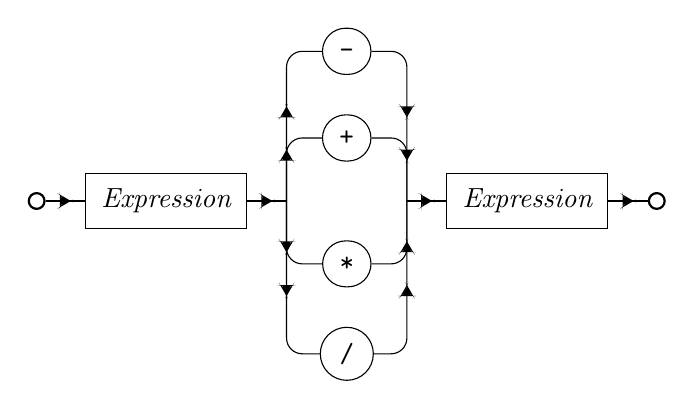
\begin{tikzpicture}
    \node[entry] (entry) {};
    \node[nterm] (left-expr) [right=of entry] {Expression};
    \coordinate [right=of left-expr] (expr-op);
    \node[term] (plus) [above right=.5cm and .75cm of expr-op] {+};
    \node[term] (minus) [above=of plus] {-};
    \node[term] (multiply) [below right=.5cm and .75cm of expr-op] {*};
    \node[term] (divide) [below=of multiply] {/};
    \coordinate [below right=.5cm and .75cm of plus] (op-expr);
    \node[nterm] (right-expr) [right=of op-expr] {Expression};
    \node[exit] (exit) [right=of right-expr] {};

    \draw[arrs] (entry) -- (left-expr) -- (expr-op);
    \draw[arr] (expr-op) |- (plus);
    \draw[arr] (expr-op) |- (minus);
    \draw[arr] (expr-op) |- (multiply);
    \draw[arr] (expr-op) |- (divide);

    \draw[arr] (plus) -| (op-expr);
    \draw[arr] (minus) -| (op-expr);
    \draw[arr] (multiply) -| (op-expr);
    \draw[arr] (divide) -| (op-expr);

    \draw[arrs] (op-expr) -- (right-expr) -- (exit);
  \end{tikzpicture}
\end{figure}

\subsection{Logical}

Logical expressions. \&\& is logical and, || (there's some weird font issue here) is logical or, and ! is logical not.

\begin{figure}[H]
  \centering
  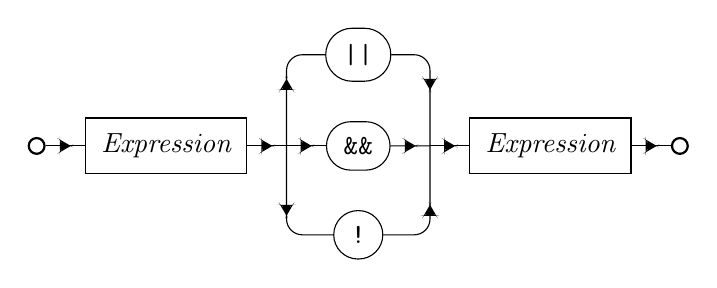
\begin{tikzpicture}
    \node[entry] (entry) {};
    \node[nterm] (left-expr) [right=of entry] {Expression};
    \coordinate [right=of left-expr] (expr-op);
    \node[term] (and) [right=of expr-op] {\&\&};
    \node[term] (or) [above=of and] {||};
    \node[term] (not) [below=of and] {!};
    \coordinate [right=of and] (op-expr);
    \node[nterm] (right-expr) [right=of op-expr] {Expression};
    \node[exit] (exit) [right=of right-expr] {};

    \draw[arrs] (entry) -- (left-expr) -- (expr-op);
    \draw[arrs] (op-expr) -- (right-expr) -- (exit);

    \draw[arr] (expr-op) -- (and);
    \draw[arr] (expr-op) |- (or);
    \draw[arr] (expr-op) |- (not);
    \draw[arr] (and) -- (op-expr);
    \draw[arr] (or) -| (op-expr);
    \draw[arr] (not) -| (op-expr);
  \end{tikzpicture}
\end{figure}

\subsection{Range}

Range expression. Both literal expressions must be of the same type.

\begin{figure}[H]
  \centering
  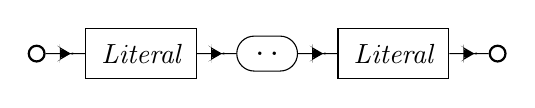
\begin{tikzpicture}
    \node[entry] (entry) {};
    \node[nterm] (lit1) [right=of entry] {Literal};
    \node[term] (dotdot) [right=of lit1] {..};
    \node[nterm] (lit2) [right=of dotdot] {Literal};
    \node[exit] (exit) [right=of lit2] {};

    \draw[arrs] (entry) -- (lit1) -- (dotdot) -- (lit2) -- (exit);
  \end{tikzpicture}
\end{figure}

\subsection{Ternary}

Ternary statement.

\begin{figure}[H]
  \centering
  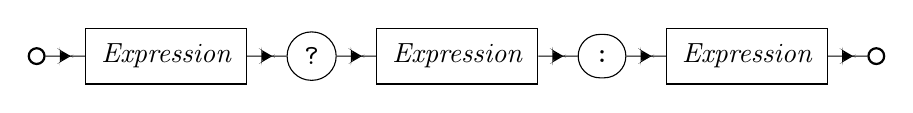
\begin{tikzpicture}
    \node[entry] (entry) {};
    \node[nterm] (expr-base) [right=of entry] {Expression};
    \node[term] (question) [right=of expr-base] {?};
    \node[nterm] (expr-true) [right=of question] {Expression};
    \node[term] (colon) [right=of expr-true] {:};
    \node[nterm] (expr-false) [right=of colon] {Expression};
    \node[exit] (exit) [right=of expr-false] {};

    \draw[arrs] (entry)
    -- (expr-base)
    -- (question)
    -- (expr-true)
    -- (colon)
    -- (expr-false)
    -- (exit);
  \end{tikzpicture}
\end{figure}

\subsection{Value}

An expression that results in a value. This is used when you need to access a value in a variable, array, or record.

\begin{figure}[H]
  \centering
  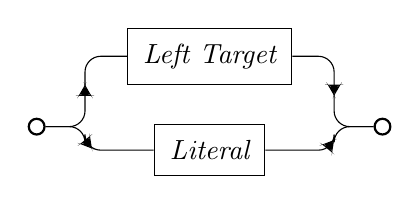
\begin{tikzpicture}
    \node[entry] (entry) {};
    \coordinate [right=of entry] (entry-list);
    \node[nterm] (target) [above right=.75cm of entry-list] {Left Target};
    \node[nterm] (literal) [below=of target] {Literal};
    \coordinate [below right=.75cm of target] (list-exit);
    \node[exit] (exit) [right=of list-exit] {};

    \draw[arr] (entry) -- (entry-list) |- (target);
    \draw[arr] (entry) -- (entry-list) |- (literal);
    \draw[arr] (target) -| (list-exit) -- (exit);
    \draw[arr] (literal) -| (list-exit) -- (exit);
  \end{tikzpicture}
\end{figure}

\end{document}

